\documentclass[ignorenonframetext,hyperref={pdftex,unicode}]{beamer}

\usepackage[T1,T2A]{fontenc}
\usepackage[utf8]{inputenc}
\usepackage[english,russian]{babel}
\usepackage{amsmath}
\usepackage{times}
\usepackage{color,graphicx,ulem,cmap}

\usepackage{beamerthemesplit}

\usepackage[unicode]{hyperref}

\mode<presentation>
{
  \usetheme{Warsaw}
  \setbeamercovered{transparent}
}

\title[Объёмные акустические волны]{Возбуждение объёмной акустической волны с поверхности кристалла парателлурита}
\author{\underline{А.С. Трушин}, П.А. Никитин}
\institute{Физический факультет МГУ им М.В. Ломоносова \\ Кафедра физики колебаний}

\begin{document}
%
\begin{frame}
\titlepage
\end{frame}
%
\begin{frame}{Постановка задачи}
  \begin{block}{Тематика}
    \begin{itemize}
    \item Почему радиофизика?
    \item Акустооптика \(\leadsto\) взаимодействие света и звука
    \item Преимущества и недостатки акустооптических приборов
    \item Метод К.Н. Баранского
    \end{itemize}
  \end{block}
  \begin{block}{Коллективы}
    \begin{itemize}
    \item ЮФУ - В.В. Роздобудько
    \item ТУСУР - С.М. Шандаров
    \item Vilnius University - D. Ciplys
    \end{itemize}
  \end{block}
\end{frame}
%
\begin{frame}{Выбор материала}
\begin{block}{Свойства материалов}
  \begin{itemize}
    \item \(TeO_2\) - рекордные акустооптические характеристики
    \item \(LiNbO_3\) - рекордный пьезоэффект
  \end{itemize}
\end{block}
\begin{columns}
  \begin{column}{5cm}
    \begin{block}{Парателлурит}
      \(d_{14} = 8.2 \cdot 10^{-12}\text{Кл}/\text{Н}\) 
      \(M_2 = 1200 \cdot 10^{-18} \text{см}^3 / \text{г}\)
      \(I\approx E^2 \cdot 8 \cdot 10^{-38} \big[\frac{\text{Кл}^2 \cdot \text{с}^3}{\text{Н}^2 \cdot \text{г}}\big]\)
    \end{block}
  \end{column}
  \begin{column}{5cm}
    \begin{block}{Ниобат лития}
      \(d_{15} = 74.0 \cdot 10^{-12}\text{Кл}/\text{Н}\)
      \(M_2 = 22,2 \cdot 10^{-18} \text{см}^3 / \text{г}\) 
      \(I\approx E^2 \cdot 16 \cdot 10^{-38} \big[\frac{\text{Кл}^2 \cdot \text{с}^3}{\text{Н}^2 \cdot \text{г}}\big]\)
    \end{block}
  \end{column}
\end{columns}
\end{frame}
%
\begin{frame}{Геометрия ячейки}
  \begin{block}{Требования к конструкции}
    \begin{itemize}
    \item Необходима мода \([110]\)
    \item Возбудить моду с поверхности \([110]\) невозможно
    \item Необходимо преобразование моды
    \end{itemize}
  \end{block}
   \begin{columns}
     \begin{column}{5cm}
       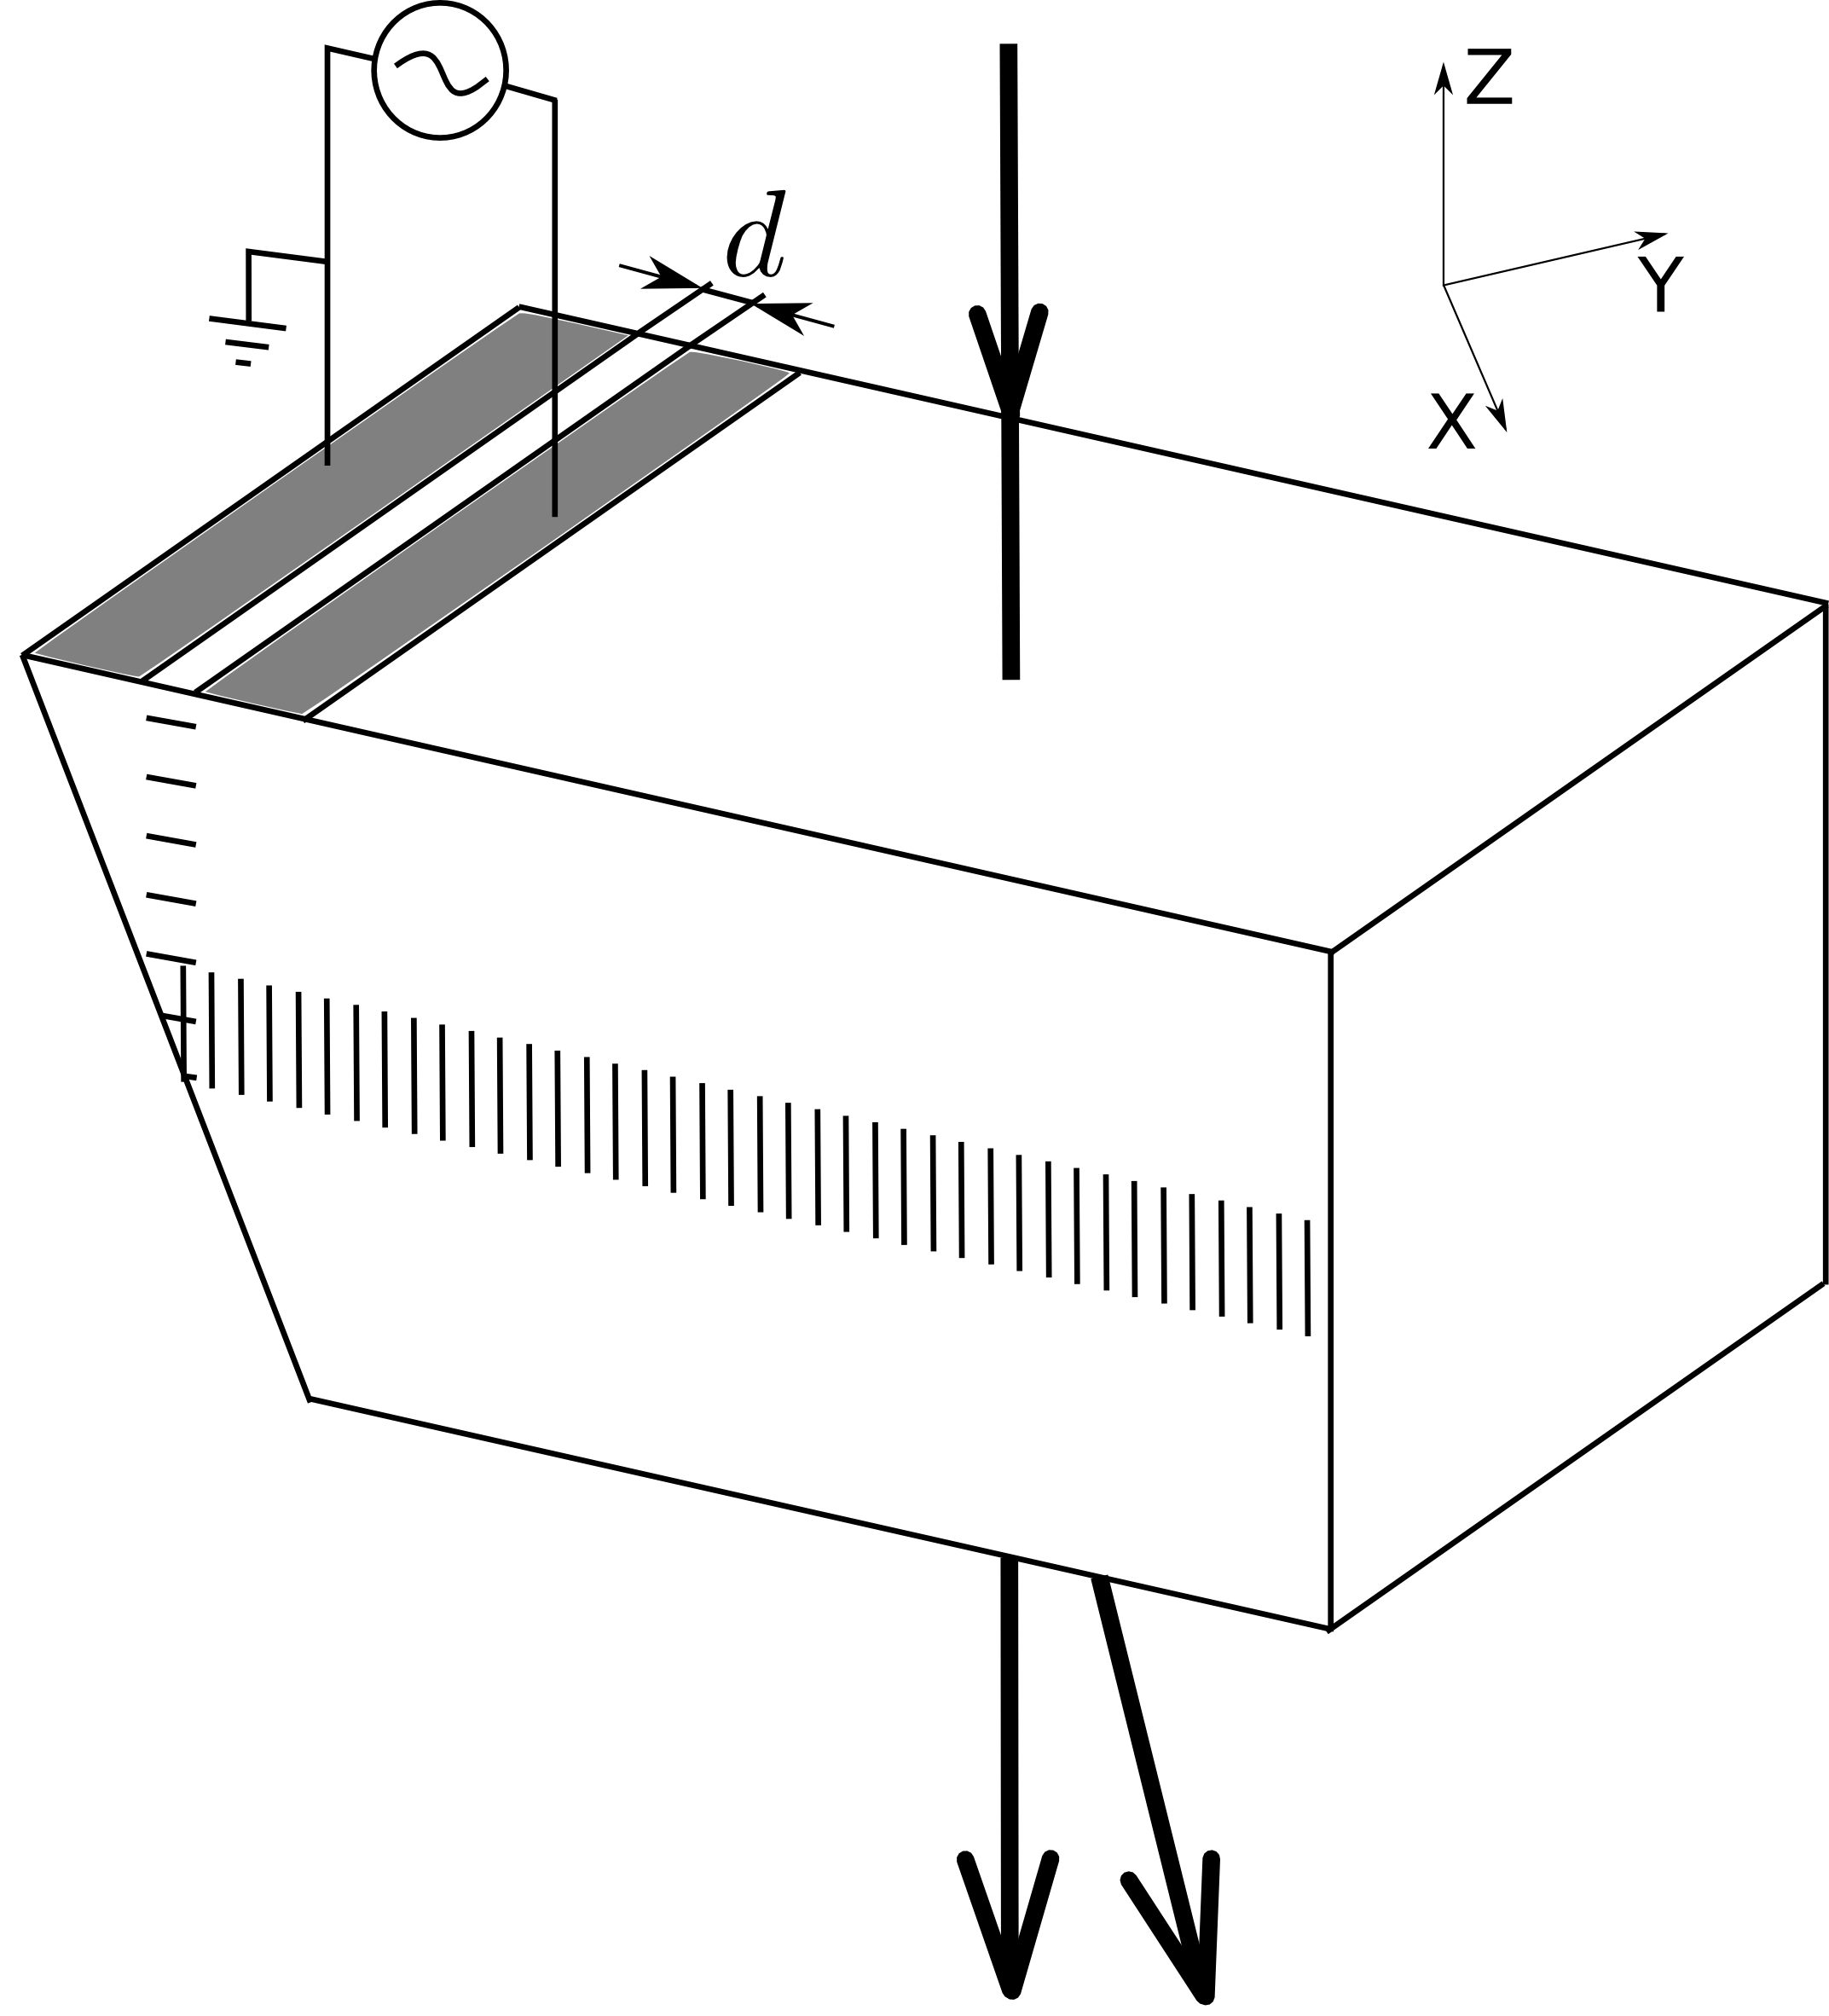
\includegraphics[width=4cm]{pictures/cell_geometry.png}
     \end{column}
     \begin{column}{5cm}
       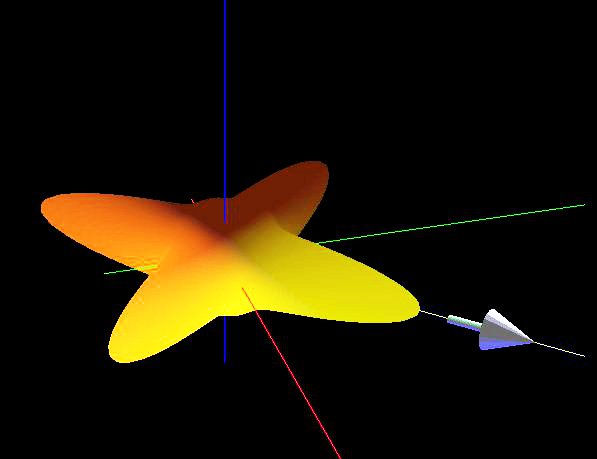
\includegraphics[width=5cm]{pictures/teo2_slowness.jpg}
     \end{column}
   \end{columns}
\end{frame}
%
\begin{frame}{Принцип работы}
  \begin{block}{Физические процессы}
    \begin{itemize}
      \item Резонанс в цепи согласования
      \item Обратный пьезоэффект
      \item Преобразование мод
      \item Акустооптическое взаимодействие
    \end{itemize}
  \end{block}
  \begin{center}
    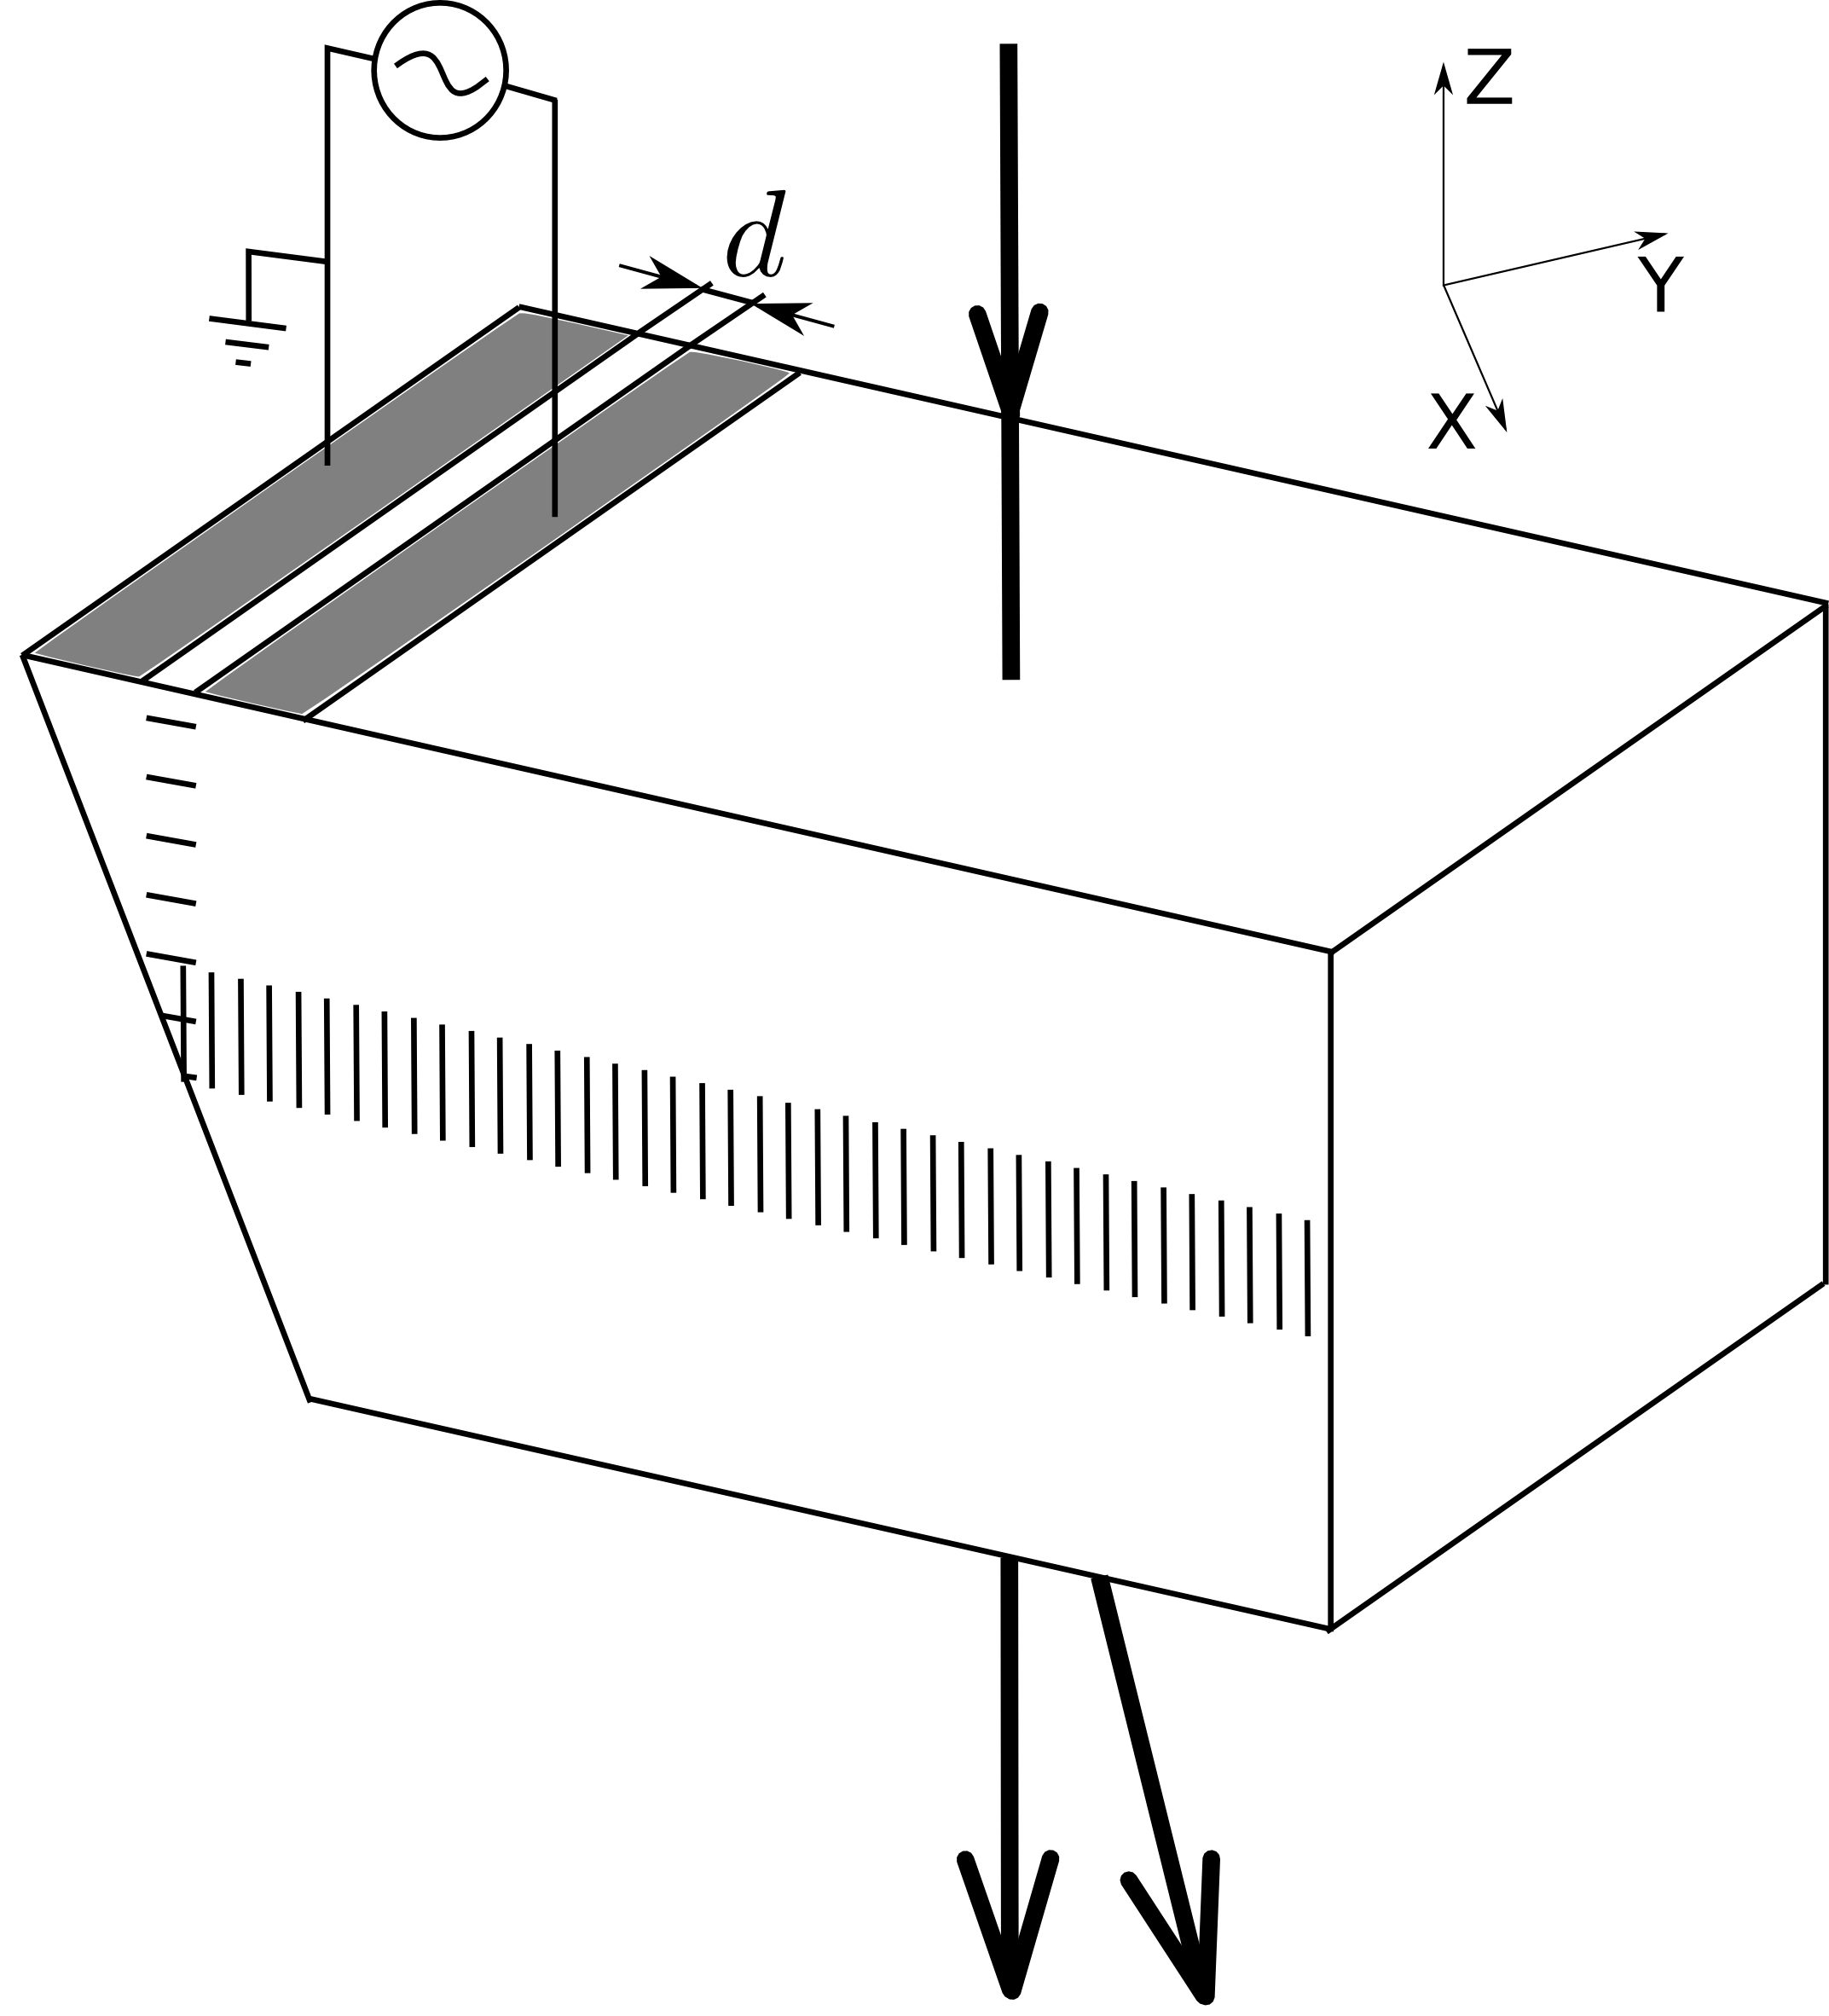
\includegraphics[width=4cm]{pictures/cell_geometry.png}
  \end{center}
\end{frame}
%
\begin{frame}{Вид экспериментального прототипа}
  \begin{block}{Акустооптическая ячейка со схемой согласования}
    \begin{columns}
      \begin{column}{5.5cm}
        \begin{center}
          ``параллельный конденсатор''
          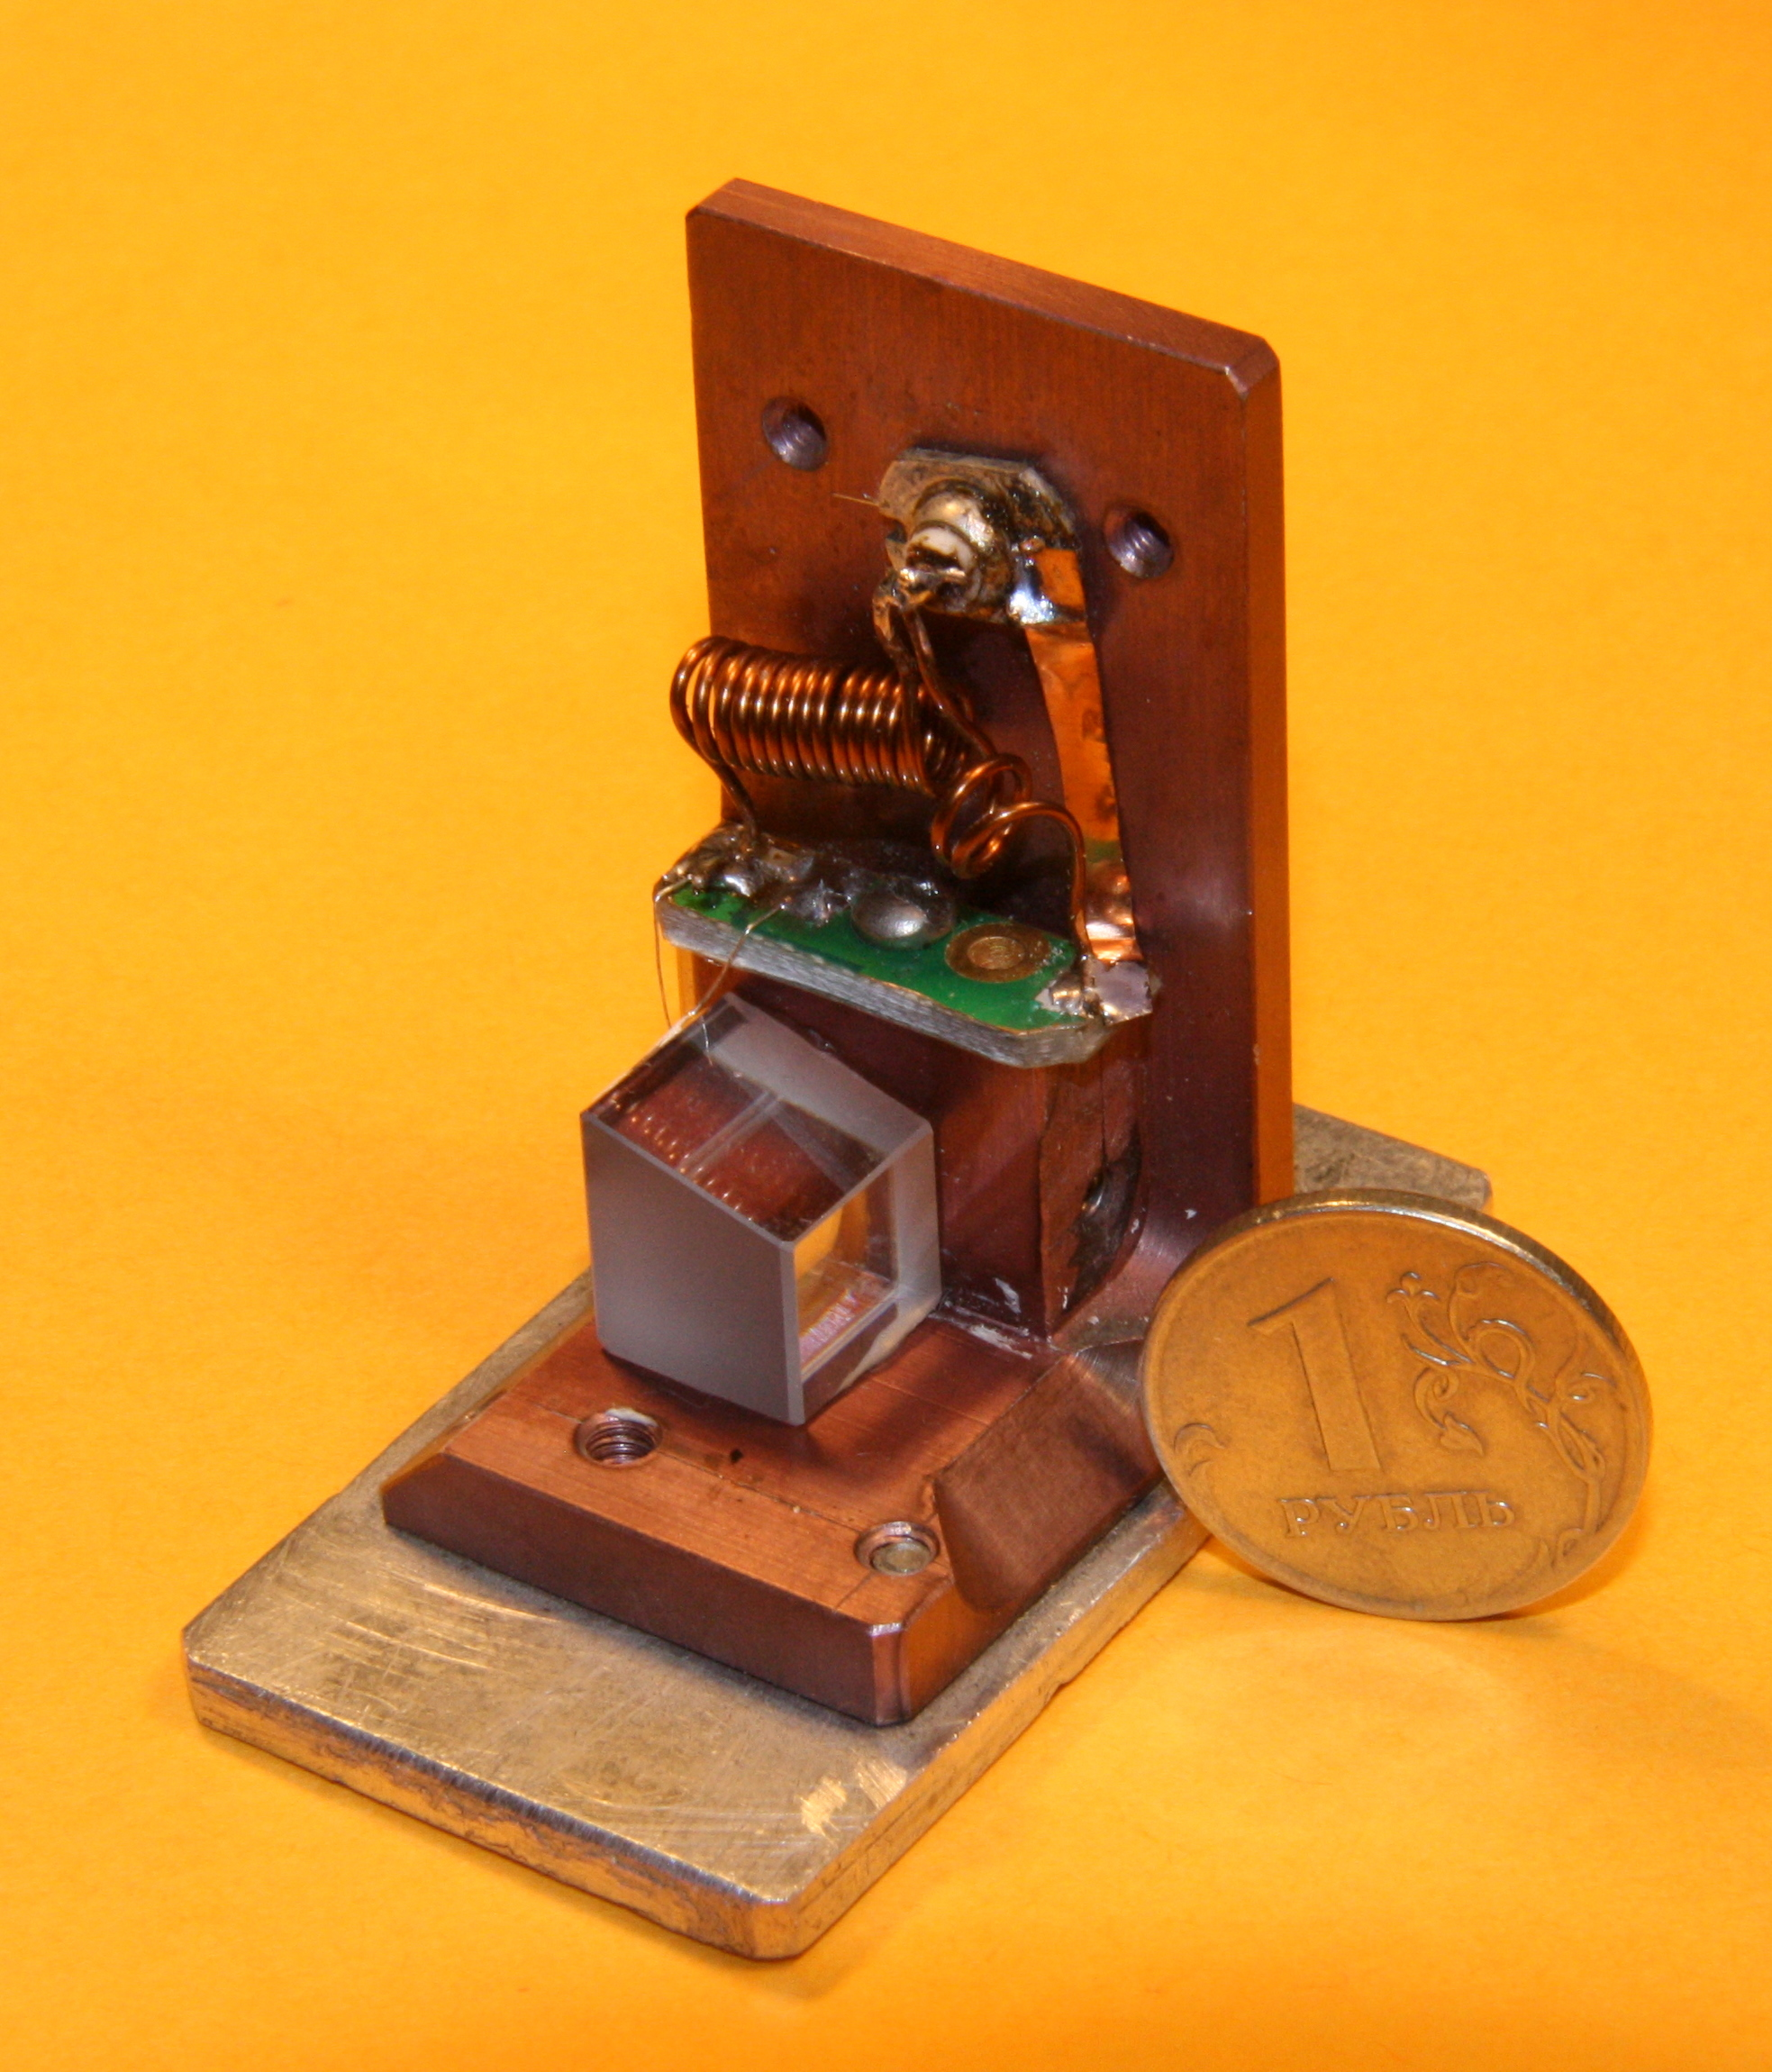
\includegraphics[height=5cm]{pictures/cell_crystal_view.jpg}
        \end{center}
      \end{column}
      \begin{column}{5.5cm}
        \begin{center}
          трансформатор
          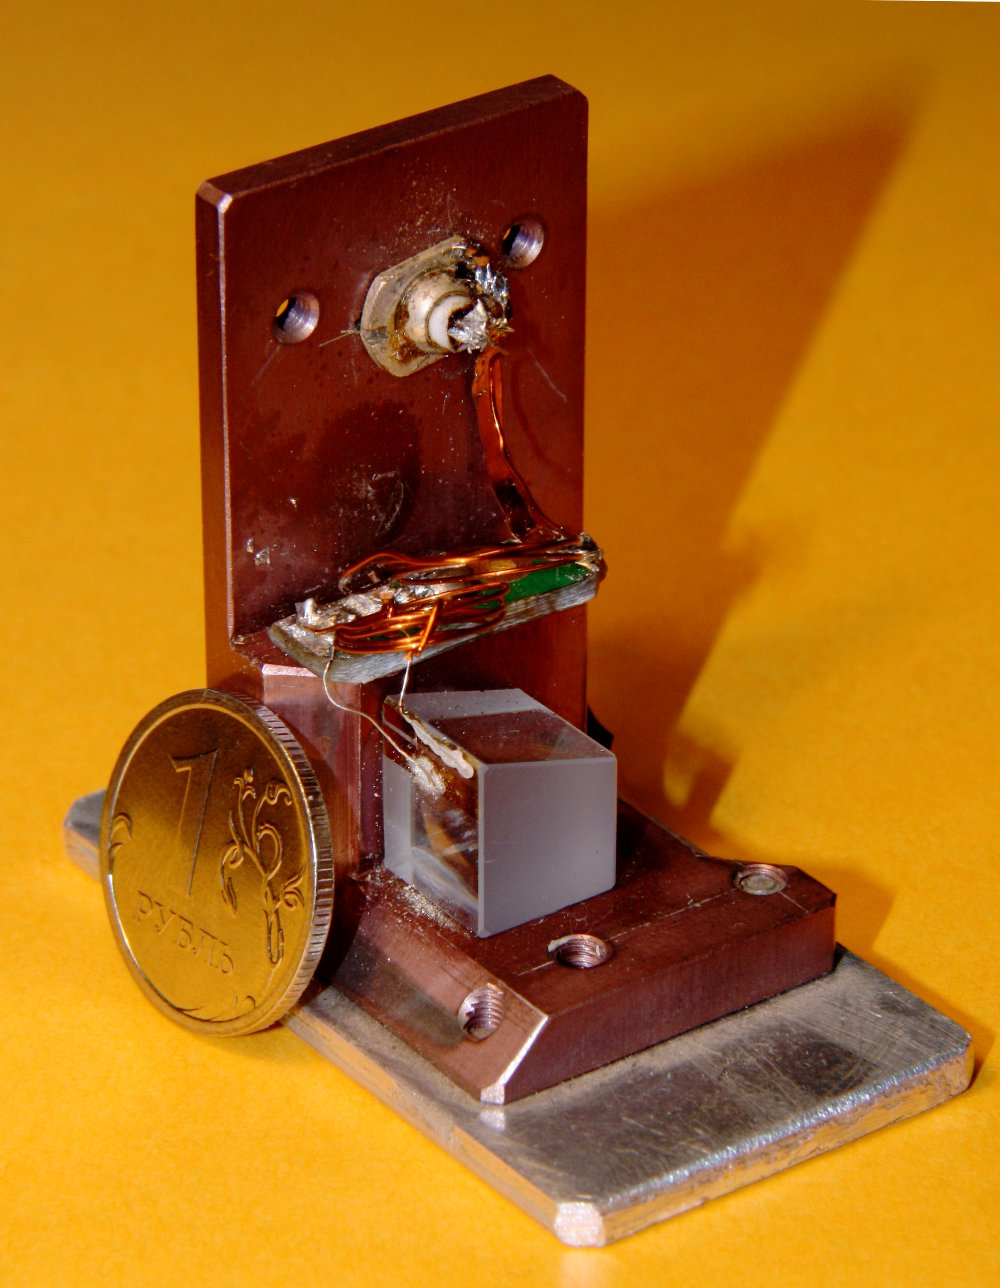
\includegraphics[height=5cm]{pictures/cell_transformator_match.jpg}
        \end{center}
      \end{column}
    \end{columns}
  \end{block}
\end{frame}
%
\begin{frame}{Эксперимент}
  \begin{center}
    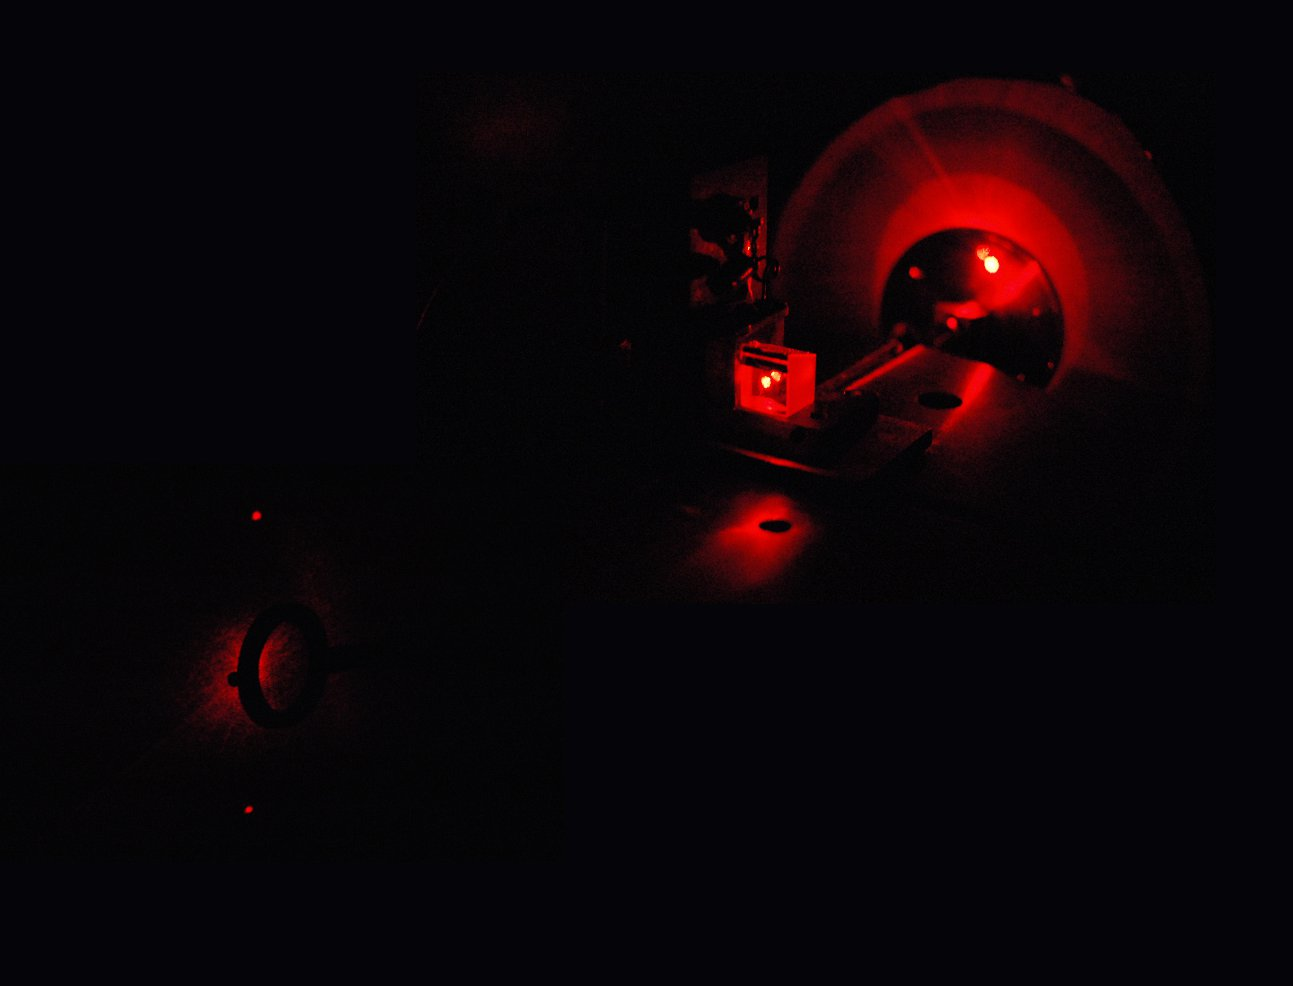
\includegraphics[width=10cm]{pictures/experiment.jpg}
    \end{center}
\end{frame}
%
\begin{frame}{Схема определения эффективной длины}
  \begin{center}
    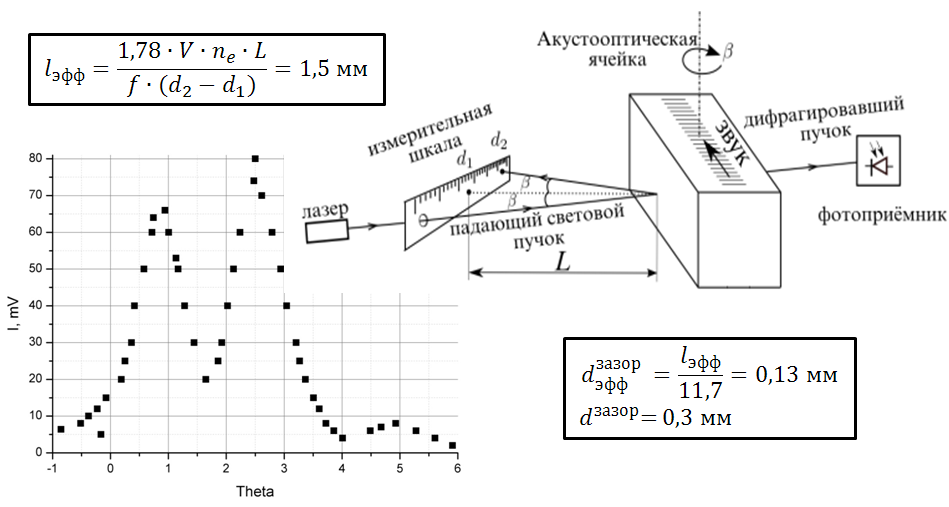
\includegraphics[width=10cm]{pictures/leff.png}
  \end{center}
\end{frame}
%
\begin{frame}{Изменение расходимости пучка при отражении}
  \begin{center}
    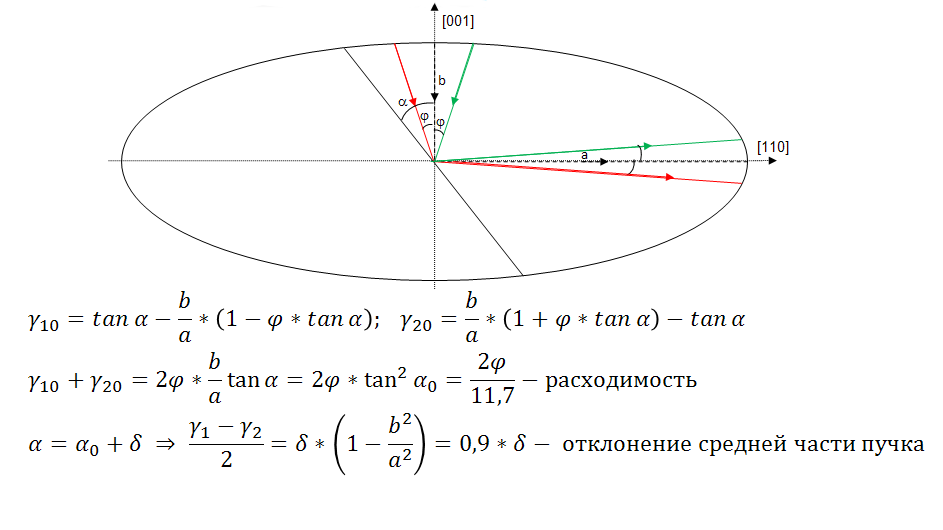
\includegraphics[width=10cm]{pictures/diverg.png}
  \end{center}
\end{frame}
%
\begin{frame}{Выводы}
  \begin{itemize}
  \item Создан лабораторный прототип акустооптического дефлектора на кристалле парателлурита с поверхностным возбуждением объёмной акустической волны
  \item Для длины волны света \(\lambda=532\)~нм и частоты управляющего сигнала \(f=70\)МГц достигнута эффективность дифракции \(\approx1\%\)~на 1~Ватт управляющей электрической мощности 
    \item При расстоянии между электродами 0.3~мм размер области возбуждения оценивается в 0.13~мм
  \end{itemize}
\end{frame}
%
\end{document}
